%!TEX root = ../egpaper_final.tex
\section{Approach}

Our pipeline is summarized in Figure \ref{overview-diagram}. We begin with a pair of RGB stereo images. From this image pair and calibration parameters obtained offline, we apply a stereo matching algorithm (See Section \ref{stereo-matching-section} to get a depthmap of the scene. Using camera instrinsic parameters, we can project this depthmap into 3D space and obtain a point cloud of the environment (See Section \ref{pointcloud-section}. Using two different methods described in Section \ref{plane-section}, we show how this point cloud can be decomposed into a set of planes. Finally, we use this set of planes to construct a polytope. The robot can then use this geometric representation of the terrain to plan its foot trajectory.


\begin{figure}[!h]
\centering
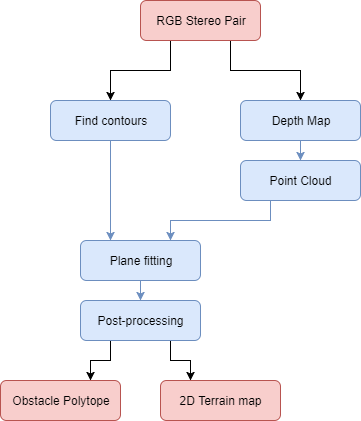
\includegraphics[width=2in]{Sections/Figures/Final-Project-Pipeline.png}
\caption{An overview of our obstacle reconstruction pipeline.}
\label{overview-diagram}
\end{figure}

\subsection{Stereo Matching} \label{stereo-matching-section}

\begin{figure}[!h]
\centering
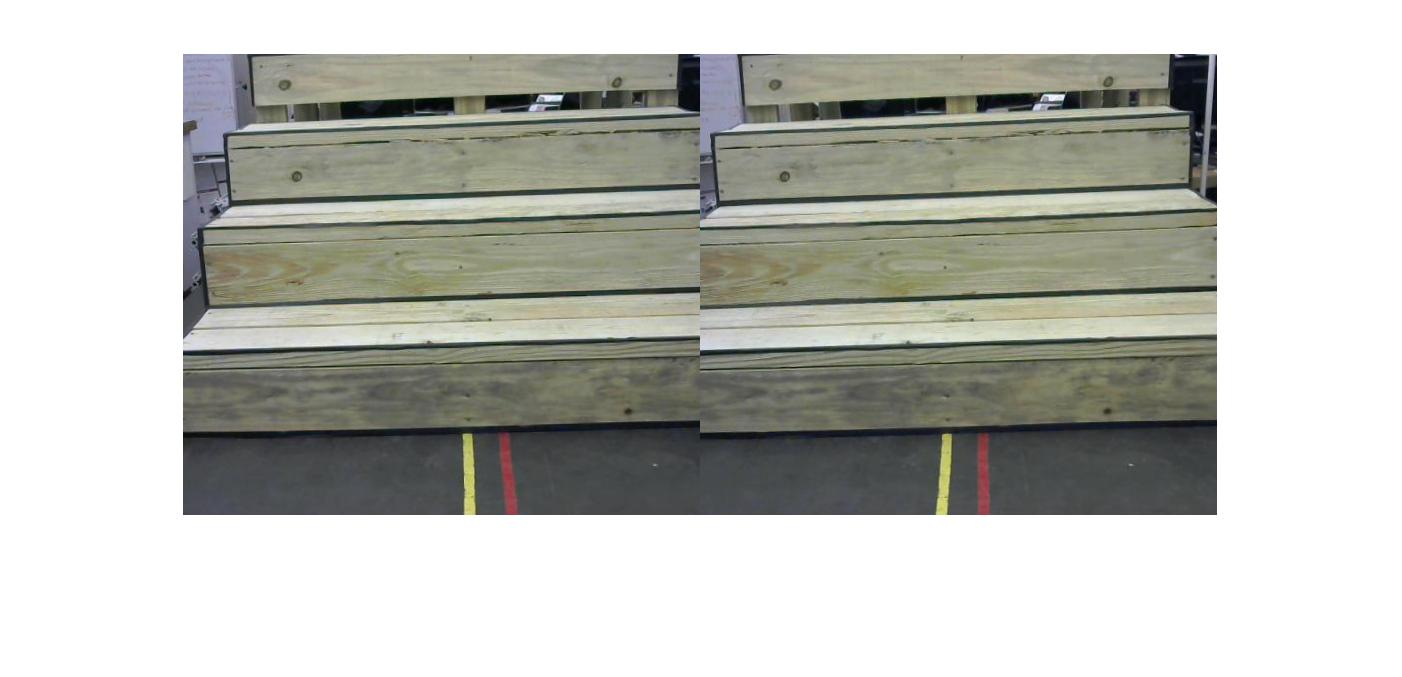
\includegraphics[width=3.3in]{Sections/Figures/example_stereo_pair.jpg}
\caption{An example stereo image pair taken by our camera setup. The two cameras are parallel and have a baseline of approximately 8cm.}
\label{stereo-image-pair}
\end{figure}

\begin{figure}[!h]
\centering
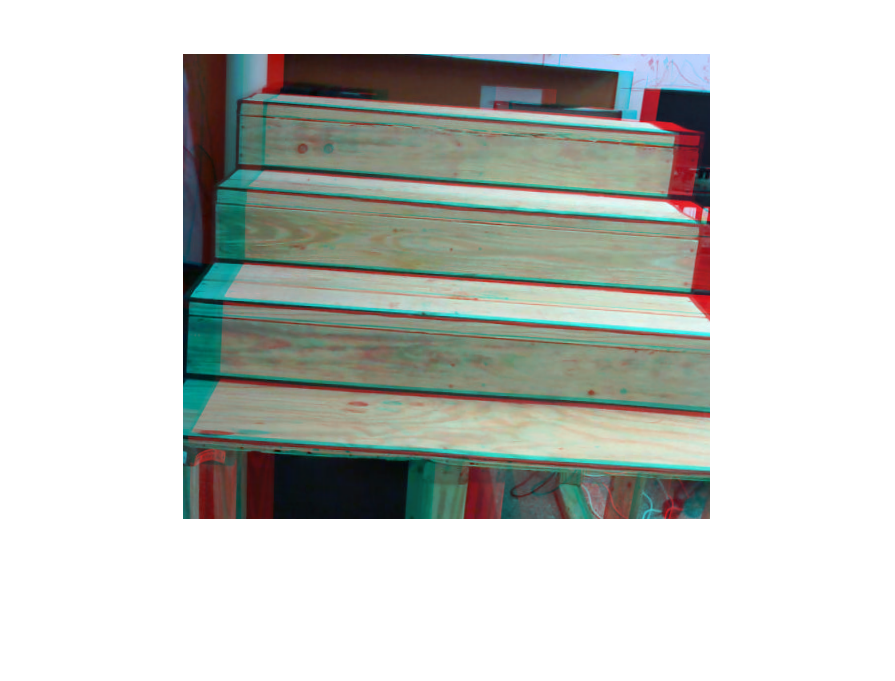
\includegraphics[width=3.3in]{Sections/Figures/stereo_anaglyph.png}
\caption{An example stereo anaglyph.}
\label{stereo-anaglyph}
\end{figure}

\subsection{Point Cloud from Depthmap} \label{pointcloud-section}

\begin{figure}[!h]
\centering
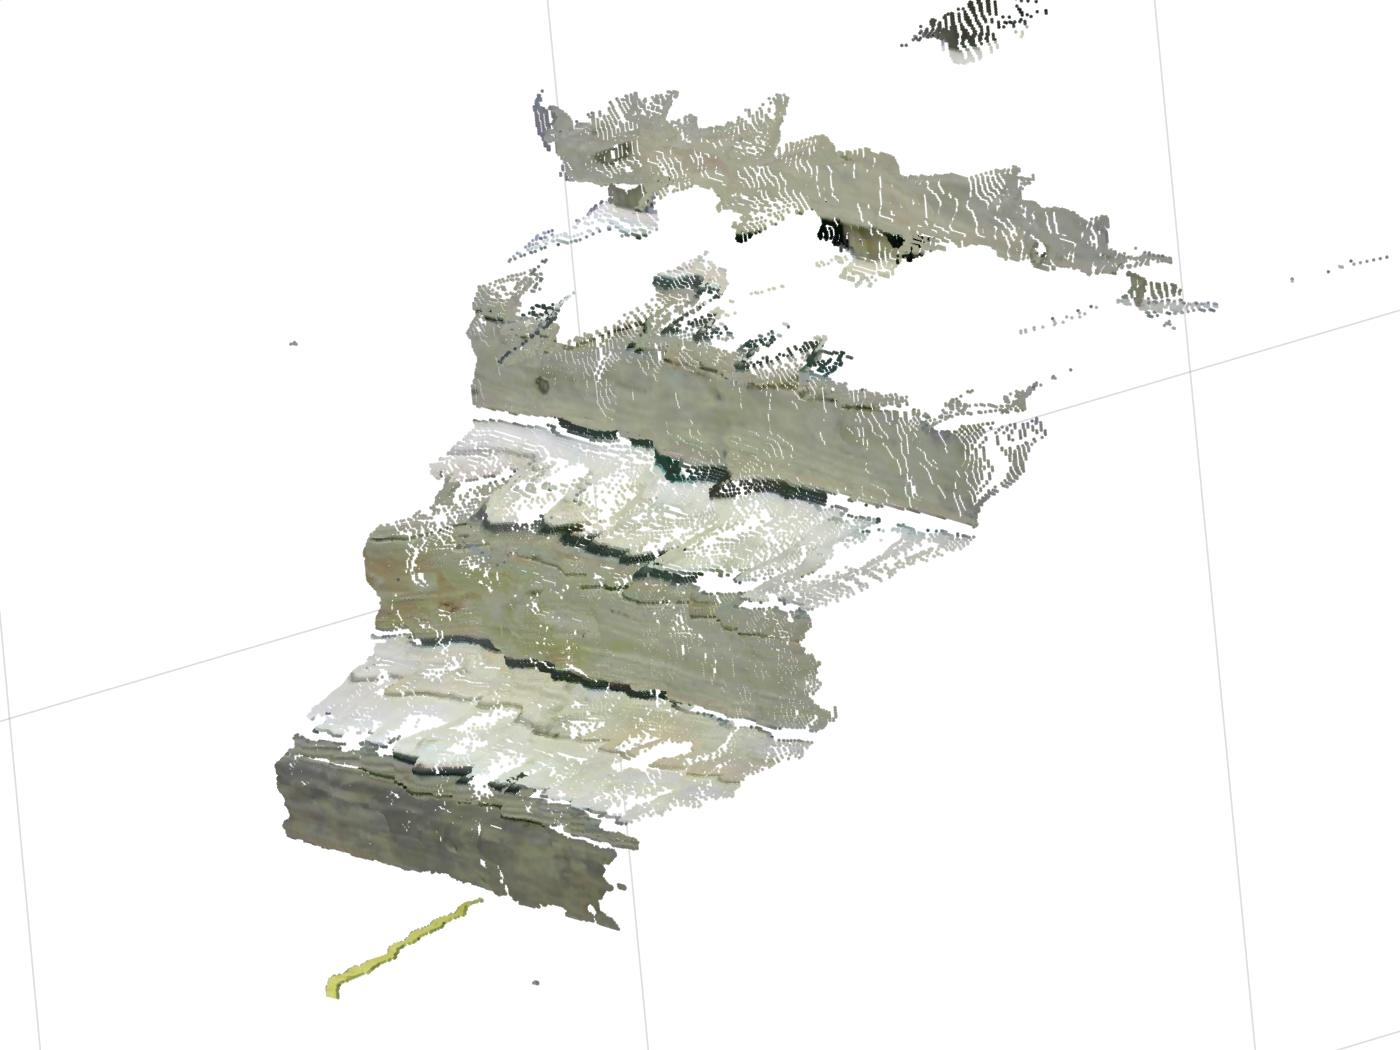
\includegraphics[width=3.3in]{Sections/Figures/example_stairs_pointcloud.jpg}
\caption{A pointcloud representation of the set of stairs in Figure \ref{stereo-image-pair}.}
\label{pointcloud-example}
\end{figure}

\subsection{Planar Decomposition of Point Clouds} \label{plane-section}

In order to estimate a polytope representation of an obstacle, we must first decompose its point cloud into a set of planes. We demonstrate two approaches for finding planes in a raw point cloud. 

In the first approach \ref{contour-method}, we find large contours in the original RGB image and project these contours into the point cloud to find subsets points that are likely to be coplanar. In the second approach \ref{orient-method}, we make the assumption that planes are either horizontal or vertical, and search for planes in the raw point cloud who are close to these orientations and are supported by many inliers. In both approaches, MSAC (M-Estimator SAmple Consensus \cite{msac-article}) is the algorithm used for plane estimation.

\subsubsection{Contour Method} \label{contour-method}

We find contours in the original RGB image using MATLAB's built in \textit{imcontour} function. Internally, this function uses the Theo Pavlidis algorithm \cite{pavlidis} to look for contours in the image at multiple levels.

Contours are then sorted by area, and pairs of contours with Intersection-over-Union (IoU) above a threshold of 0.3 are replaced by the larger of the two contours. Highly overlapping contours are likely to lie on the same plane, and we observed empirically that our reconstruction performs better when there are no duplicate planes.

We then project our candidate contours into the point cloud, and find 3D points that originally from inside of this contour in the RGB image. A plane is fit to each planar subset of the point cloud using MSAC with no reference normals.

\begin{figure}[!h]
\centering
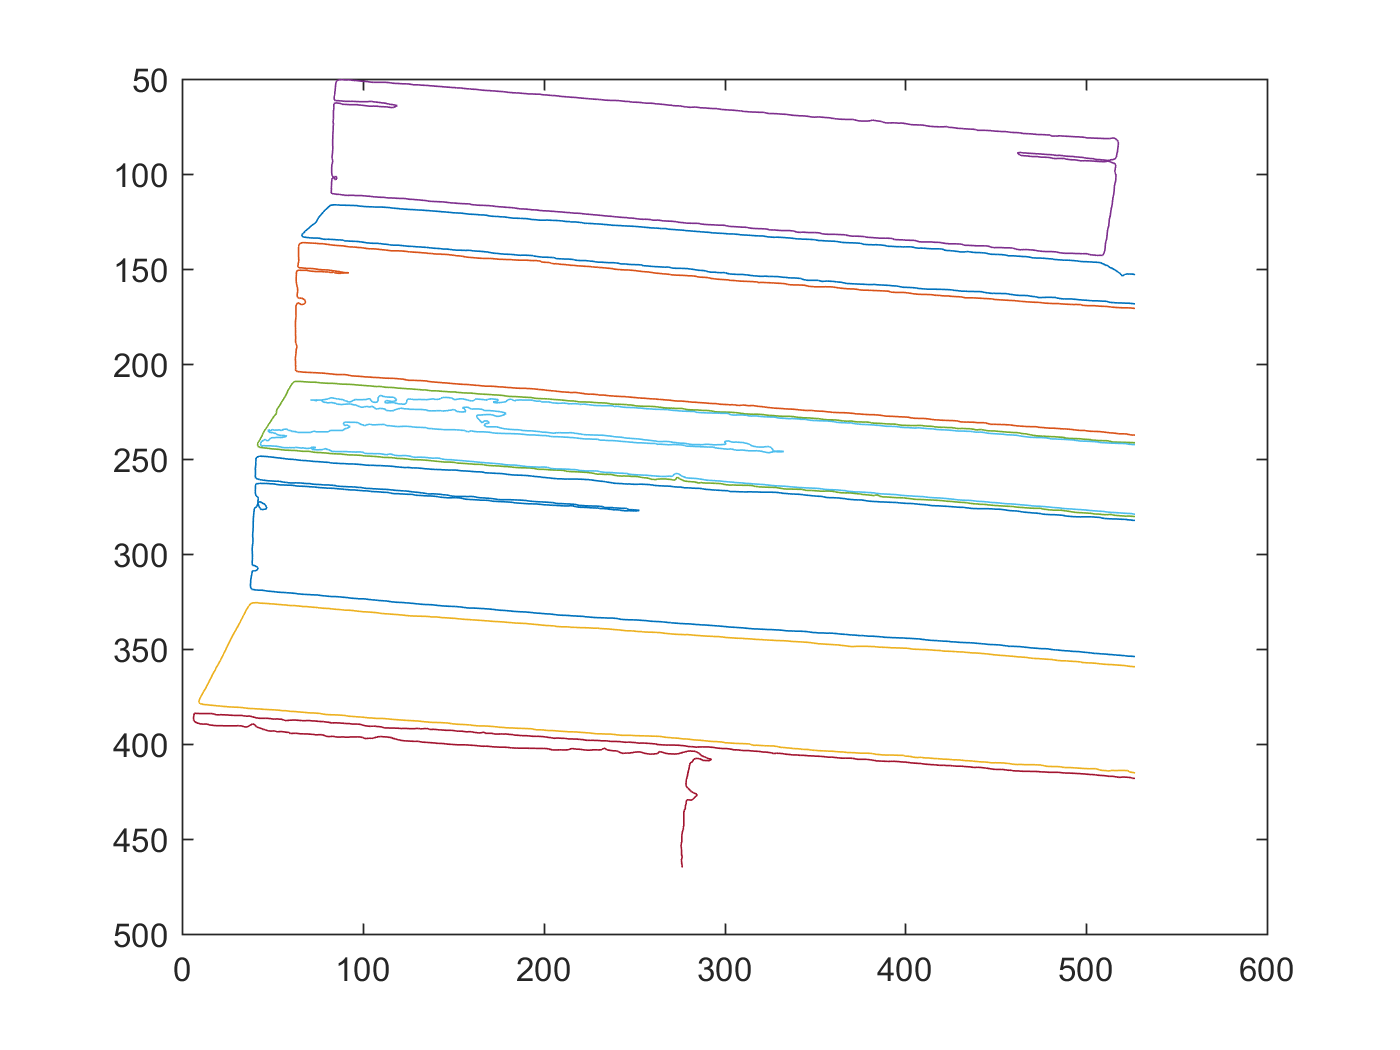
\includegraphics[width=3.3in]{Sections/Figures/good_contour_plot_12-7.png}
\caption{An example contour plot of the stairs in Figure \ref{stereo-anaglyph}. Here we have shown the eight largest contours in the image by area.}
\label{contours-example}
\end{figure}

\subsubsection{Orientation Method} \label{orient-method}

The Contour Method, as one might expect, is highly sensitive to lighting effects and the sharpness of edges on the obstacle. In order to provide robustness to lighting conditions and the visual characteristics of the obstacle, we propose an orientation method for plane fitting that does not depend on contours.

In this method, we assume that the obstacle is composed of a predetermined number of horizontal and vertical planes in the world frame. During MSAC, we sample three points from the point cloud and compute the parameters of a plane with them. We require that the normal of this plane is within an angular tolerance of a reference normal vector (i.e the z-axis for vertical planes and the y-axis for horizontal planes). If the robot frame is not aligned with the world frame, we can rotate our reference normals before performing this step. Ultimately, MSAC finds a plane that is very close to horizontal or vertical, and has the lowest cost based on inliers and outliers. We then remove the inlier points from the point cloud, and iteratively fit horizontal and vertical planes to the residual point cloud. Although our algorithm currently looks for a fixed number of planes, it would be simple to add a condition that stops extracting planes once there are insufficient supporting inliers.

\subsection{Polytope Reconstruction from Unordered Planes} \label{polytope-section}

At this stage in the pipeline, we have an unordered set of planes, each represented by four parameters: a surface normal and offset constant. There are many ways that these planes could intersect to form a polytope, but only one that actually matches our ground truth observation. We must make another assumption here about the composition of the polytope.

When using the Contour Method in Section \ref{contour-method}, we assume that the depth and height ordering of planes in 3D space is given by the vertical ordering of planes in the RGB image. Horizontal planes that appear higher in the RGB image are also higher in the scene. Similarly, vertical planes that appear higher in the RGB image are deeper in the scene.

\begin{figure}[!h]
\centering
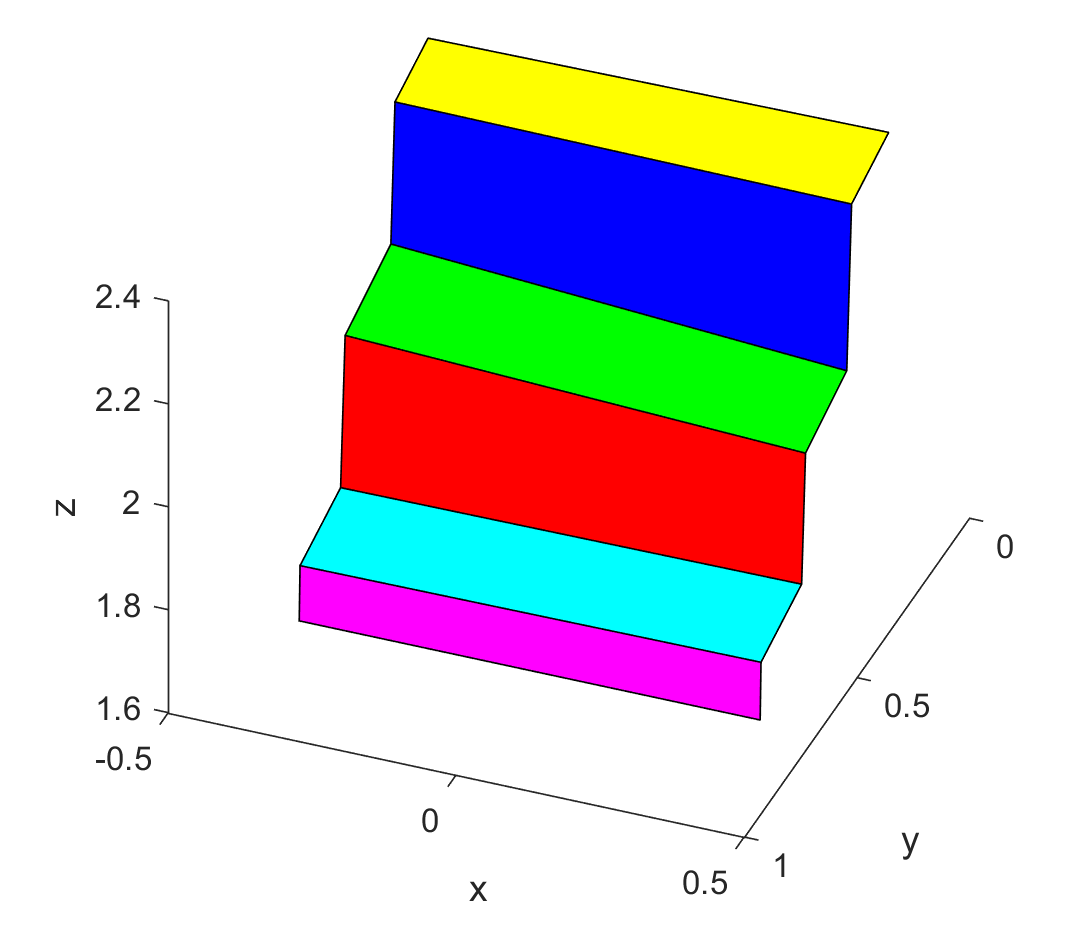
\includegraphics[width=3.3in]{Sections/Figures/polytope_example.png}
\caption{A polytope reconstruction of the image in Figure \ref{stereo-image-pair}, using the Contour Method (See Section \ref{contour-method}). The pink, red, and blue planes correspond to horizontal faces of the stairs. The light-blue, green, and yellow planes are vertical faces.}
\label{polytope-diagonal-contour}
\end{figure}

\begin{figure}[!h]
\centering
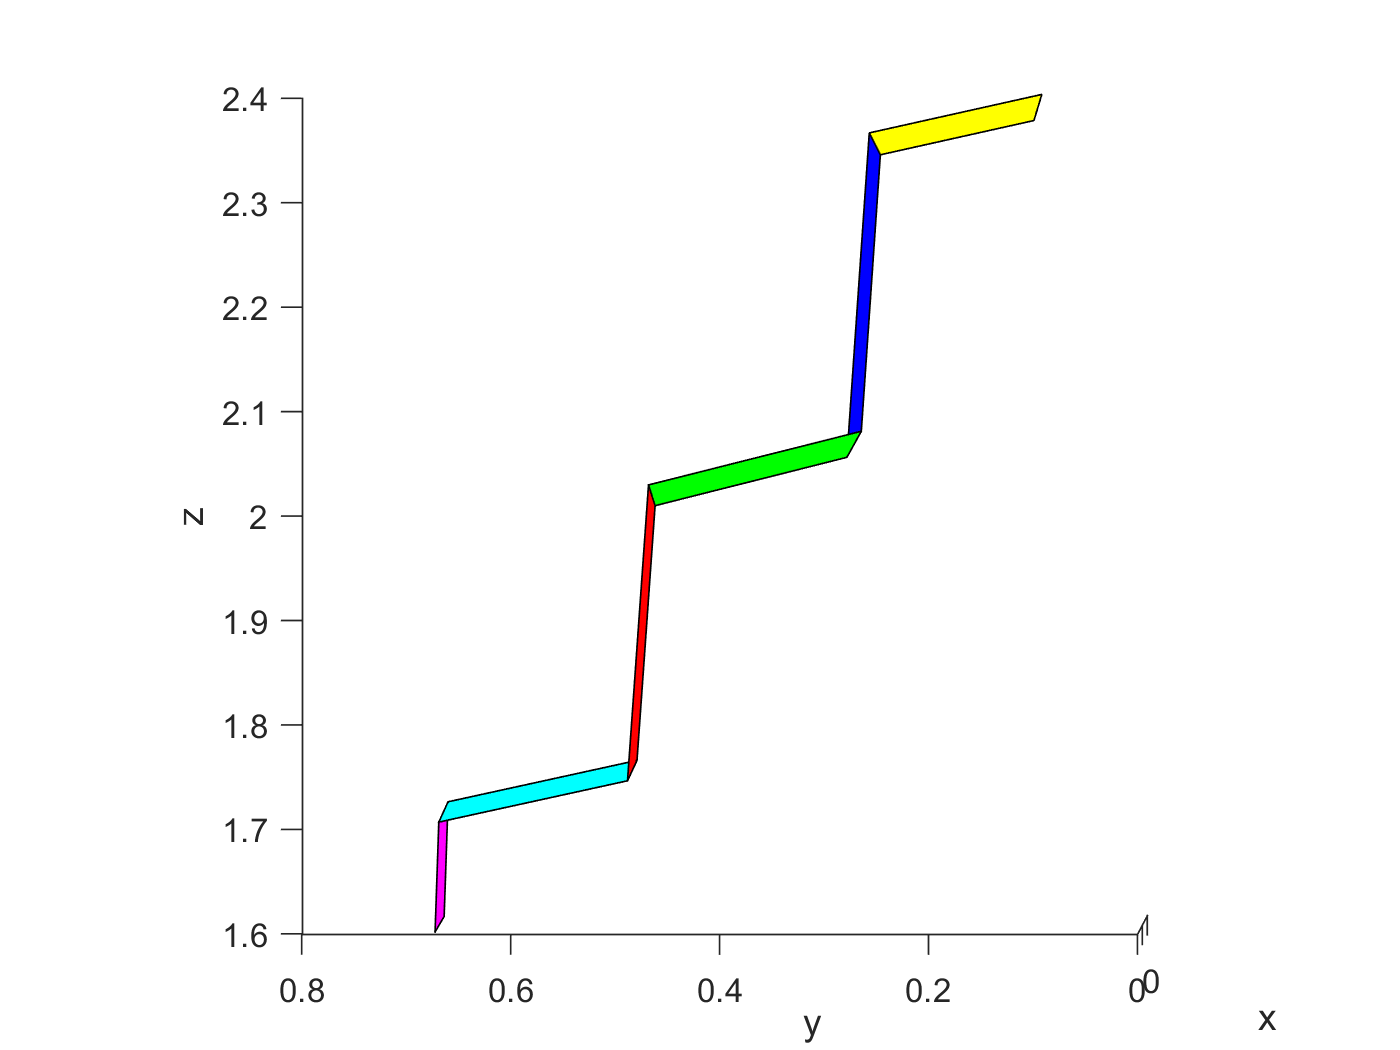
\includegraphics[width=3.3in]{Sections/Figures/polytope_sideview.png}
\caption{The polytope from Figure \ref{polytope-diagonal-contour} viewed from the side. The vertical faces of this polytope (light-blue, green, yellow) are very close to the groundtruth dimension of 20cm. Similarly, the remaining horizontal faces are close to their groundtruth dimension of 31cm. Note that the pink plane is cut off by a bounding box around the polytope, so it does not appear to be the correct size.}
\label{polytope-sideview-contour}
\end{figure}

When using the Orientation Method in Section \ref{orient-method}, we use a sampling based approach to order planes. We sort all vertical planes based on their distance from the camera, then find the horizontal plane that is ``active'' between each pair of vertical planes. The ``active'' horizontal plane is the one that has the smallest average distance to a sample of points in the region between the vertical planes.

\begin{figure}[!h]
\centering
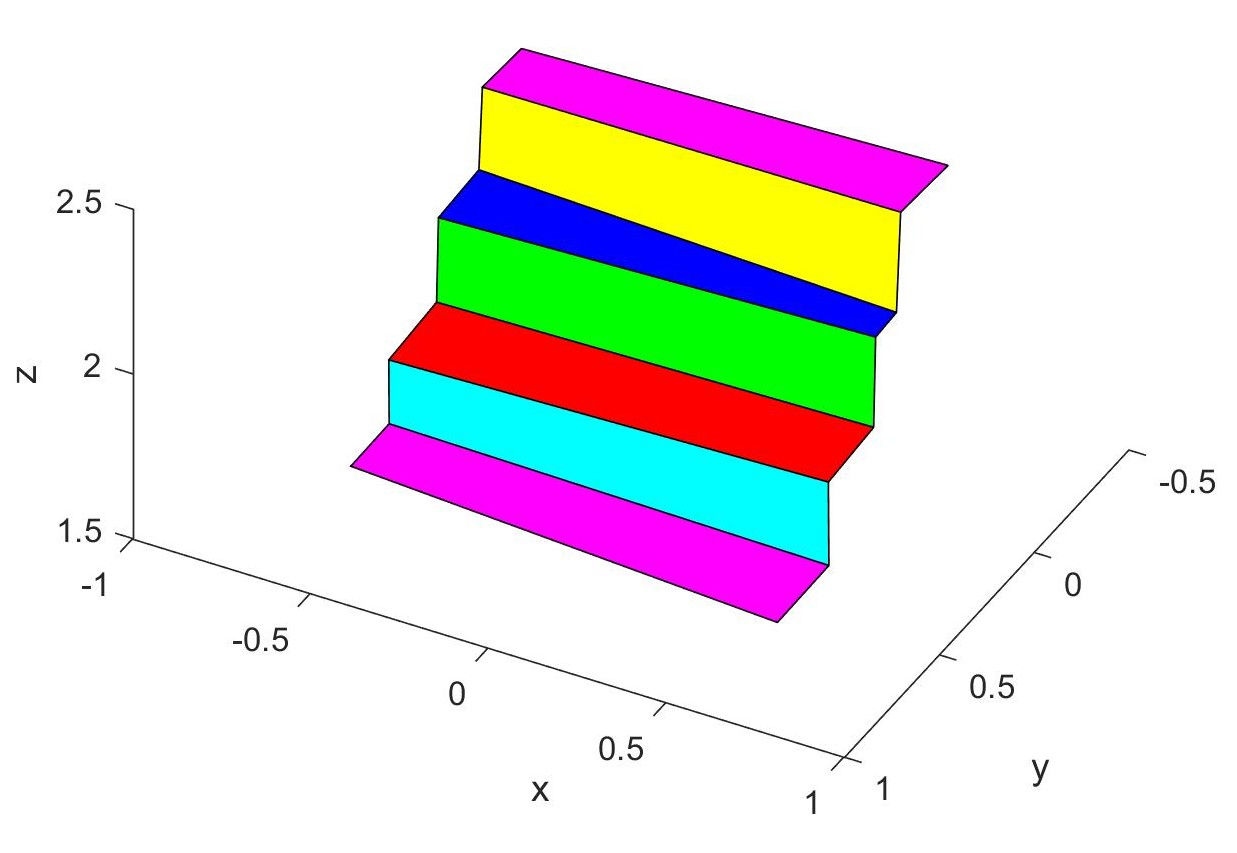
\includegraphics[width=3.3in]{Sections/Figures/polytope_diagonal_geom.jpg}
\caption{A polytope reconstruction of the image in Figure \ref{stereo-image-pair}, using the Orientation Method (See Section \ref{orient-method}). Here, the pink, red, and blue planes are vertical, and the light-blue, green, and yellow are horizontal. Because the orientation method is not limited by image contours, we are able to construct a polytope with more faces than in Figure \ref{polytope-diagonal-contour}}.
\label{polytope-diagonal-orient}
\end{figure}

\begin{figure}[!h]
\centering
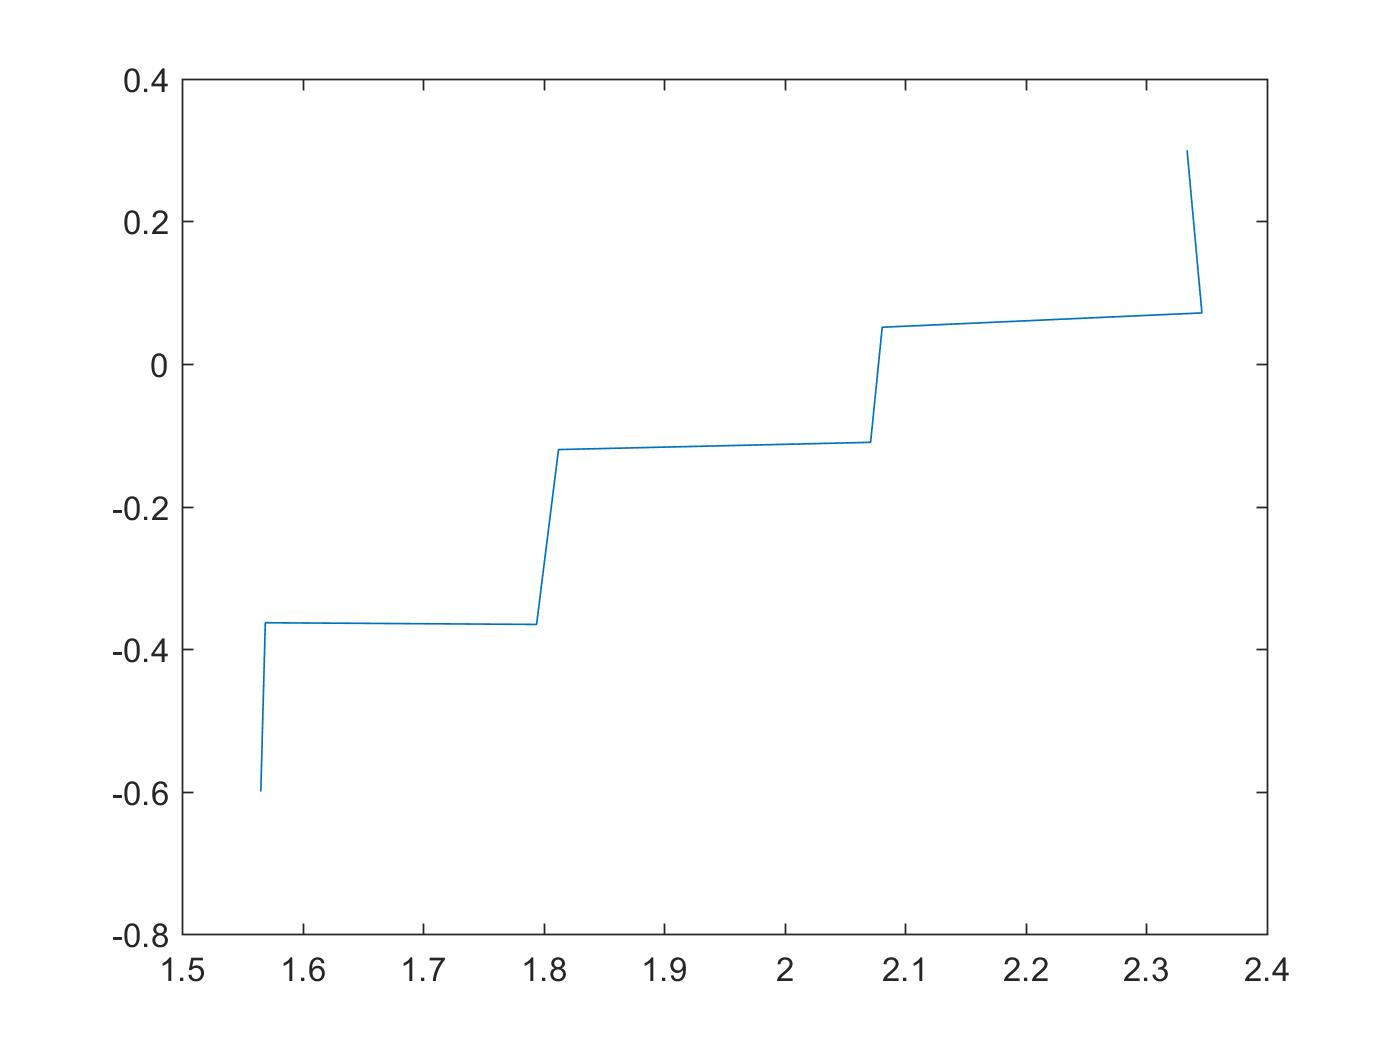
\includegraphics[width=3.3in]{Sections/Figures/geom_sideview_2d.jpg}
\caption{The polytope from Figure \ref{polytope-diagonal-orient} viewed from the side. Again, we see that vertical and horizontal planes are close to the groundtruth dimensions of 20cm and 31cm, respectively.}
\label{polytope-sideview-orient}
\end{figure}

Finally, once an ordering of planes has been established, we can compute lines of intersection between these planes, and obtain a set of vertices for the polytope. See Figures \ref{polytope-diagonal-contour} and \ref{polytope-diagonal-orient} for example reconstructions. See Figures \ref{polytope-sideview-contour} and \ref{polytope-sideview-orient} for a metric comparison of our reconstructions to groundtruth.
